\documentclass[sigplan,10pt,anonymous,nonacm]{acmart}
% EuroSys 2027 encourages ACM SIGPLAN format.  The conference CFP requires
% two columns, a 7 x 9 inch text block, >= 10 pt text on >= 12 pt leading,
% and numbered pages.  No font files are included in this source bundle.
\usepackage{amsmath,mathtools,amsthm}
\usepackage{array,tabularx,booktabs}
\usepackage{algorithm}
\usepackage{algpseudocode}
\usepackage{enumitem}
\usepackage{tikz}
\usetikzlibrary{arrows.meta,positioning,calc}
\usepackage{xurl}
\usepackage{balance}
\geometry{reset,paperwidth=8.5in,paperheight=11in,twoside,inner=0.75in,outer=0.75in,top=1in,bottom=1in,columnsep=0.34in,headheight=13pt,headsep=12pt,footskip=24pt,includeheadfoot=false}
\settopmatter{printacmref=false,printccs=false,printfolios=true}
\setcopyright{none}
\citestyle{acmnumeric}
\hypersetup{hidelinks,pdfauthor={Anonymous Author(s)},pdfsubject={Anonymous research manuscript}}
\makeatletter
% ACM's smaller ancillary sizes are raised to the EuroSys minimum.
\renewcommand\small{\@setfontsize\small{10}{12}}
\renewcommand\footnotesize{\@setfontsize\footnotesize{10}{12}}
\renewcommand\bibfont{\normalfont\fontsize{10}{12}\selectfont}
\makeatother
\captionsetup{font=normalsize,labelfont=bf,textfont=normalfont}
\algrenewcommand\alglinenumber[1]{\normalfont\fontsize{10}{12}\selectfont #1:}
\setlist[enumerate]{leftmargin=*,topsep=3pt,itemsep=2pt,parsep=0pt}
\setlist[itemize]{leftmargin=*,topsep=3pt,itemsep=2pt,parsep=0pt}
\setlength{\emergencystretch}{1em}
\newtheorem{theorem}{Theorem}[section]
\newtheorem{lemma}[theorem]{Lemma}
\newtheorem{proposition}[theorem]{Proposition}
\theoremstyle{definition}
\newtheorem{definition}[theorem]{Definition}
\newcommand{\rai}{\textsc{Rai}}
\newcommand{\NC}{\mathsf{NC}}
\newcommand{\FC}{\mathsf{FC}}
\newcommand{\FF}{\mathsf{FF}}
\newcommand{\TC}{\mathsf{TC}}
\newcommand{\Build}{\mathsf{BuildState}}
\newcommand{\Agree}{\mathsf{CheckpointAgree}}
\newcommand{\Root}{\mathsf{Root}}
\newcommand{\Replay}{\mathsf{Replay}}
\newcommand{\Final}{\mathsf{Final}}
\newcommand{\Anc}{\mathsf{Anc}}
\newcommand{\keys}{\mathsf{keys}}
\newcommand{\Sign}{\mathsf{Sign}}
\newcommand{\ctx}{\mathsf{ctx}}
\newcommand{\Send}{\mathsf{Send}}
\newcommand{\Receive}{\mathsf{Receive}}
\newcommand{\tagR}{\mathsf{R}}
\newcommand{\tagN}{\mathsf{N}}
\newcommand{\tagF}{\mathsf{F}}
\newcommand{\pending}{\mathsf{pending}}
\newcommand{\installed}{\mathsf{installed}}
\newcommand{\Byz}{\mathsf{Byz}}
\newcommand{\Compat}{\mathsf{Compatible}}
\newcommand{\EPB}{\mathsf{EPB}}
\newcommand{\para}[1]{\paragraph{#1}}
\newcolumntype{Y}{>{\raggedright\arraybackslash}X}

\title[RAI: Preserving Latent Finality Across Reconfiguration]{RAI: Preserving Latent Finality Across Committee Reconfiguration}
\author{Anonymous Author(s)}
\renewcommand{\shortauthors}{Anonymous Author(s)}
\begin{document}
\begin{abstract}
Single-writer payments can finalize from account-local quorums without a continuously agreed transaction sequence. Replacing their validator committee nevertheless requires a global boundary that preserves obligations left by old votes. A snapshot of observed final certificates is insufficient: signatures already released by the closing committee may form a certificate only after the checkpoint has been selected. We call this obligation \emph{latent finality}. RAI separates recovering such obligations from agreeing on a checkpoint. Each outgoing validator freezes a signed report committing to a tagged ledger set and to voted-for block hashes outside that ledger. A deterministic construction reconstructs selected reports, preserves explicit finality, carries recovery locks, and allows a decided checkpoint to promote a uniquely retained closing-epoch notarized prefix to finality. Immutable validation inputs make candidate reconstruction independent of later private evidence. Lagged committees permit successor preparation and restricted, prefix-wide dual-notarization overlap; arbitrary fresh successor work remains provisional until its predecessor checkpoint is known. A checkpoint-base/live-overlay invariant preserves already applied finality during installation. We give safety arguments and conditional termination results under explicit static-fault, retained-data, and progress assumptions. The contribution is a closure protocol for account-local finality, not a new consensus algorithm. A single-host RsNano prototype keeps the median non-fork latency near 100\,ms across three checkpoints and settles forked workloads, with one offline or one Byzantine validator, that the unmodified node does not finish; a Byzantine forked workload exposed and let us repair a report-checking defect the termination argument does not tolerate.
\end{abstract}
\maketitle
\section{Introduction}
\label{sec:intro}
Single-writer value transfer does not require every payment to occupy a position in a global transaction sequence. An account owner determines the order of its updates; validators must prevent incompatible owner-signed histories from becoming final. The consensus-number characterization of asset transfer formalizes this distinction, and payment systems already exploit it~\cite{consensusnumber,fastpay,astro}. The challenge addressed here is not ordinary consensus avoidance. It is replacing the validators that have been issuing account-local votes.

A reconfiguration must determine which old outcomes the successor is obliged to preserve. Consider a payment for which enough old validators have released signatures to establish finality. Network delays keep these signatures distributed, so a checkpoint builder sees no final certificate. If the checkpoint omits the payment and allows an incompatible successor history, the delayed signatures can subsequently establish a valid old-epoch final outcome. Agreement has selected a unique snapshot, but not a safe one.

We call an eligible outcome \emph{latent-final} when the released signatures suffice for a final certificate, whether or not a correct process has assembled it. More generally, closure must preserve outcomes that can still become certified using signatures from validators that have not yet stopped. An immutable report quorum must expose enough obligations to cover both cases. The relevant boundary is therefore not ``which certificates did this proposer observe?'' but ``which outcomes can the old voting domain still justify?''

RAI separates \emph{closure}, which recovers these obligations, from \emph{checkpoint agreement}, which chooses among safe candidates. A closing validator stops account signing and freezes one report containing two authenticated roots. The first commits to its ledger with distinct recovery-protected, notarized, and finalized tags. The second commits to hashes of blocks for which it voted but which are absent from that frozen ledger. Reports do not contain certificate objects. Validators retain and gossip blocks and signed votes, from which every verifier assembles quorum evidence locally.

A candidate selects $N-f$ usable reports. The deterministic procedure $\Build$ preserves inherited and explicitly exposed finality, carries represented notarization locks, and recovers a potentially fast-final branch from sufficient reporter first votes. After mandatory retention, a decided checkpoint may additionally finalize the maximal uniquely retained prefix whose blocks each have a verified closing-epoch $\NC$. Recovery-only uniqueness remains nonfinal. The crucial property is universal over valid report selections: different candidates may retain different nonfinal work, but none may discard a branch on which eligible late finality can act.

This design specializes entirely to owner-ordered sends and receives. It does not provide arbitrary shared-object transactions or atomic operations across independent writers. Sui Lutris, in contrast, combines owned-object execution with consensus for shared objects and checkpoint sequencing~\cite{lutris}. RAI's narrower application permits epoch-level agreement, but that choice alone is not novel. Its contribution is the report-based preservation argument required when there is no continuous certificate sequence to drain.

\para{Contributions.}
First, RAI specifies and establishes a report-exposure invariant for latent and late account finality. Second, it gives a deterministic, evidence-committed checkpoint construction that separates recovery locks from a narrow checkpoint-finality rule for uniquely retained notarized prefixes and reconciles checkpoint state with live finality. Third, it composes that construction with lagged committees and a restricted cross-epoch overlap rule. The closing committee decides one valid checkpoint; the already known successor independently verifies and installs it. An existing Kudzu-based voting construction supplies agreement~\cite{kudzu}; its mechanics and the single-writer restriction are not claimed as new contributions.

\para{Scope of the claims.}
The main protocol uses a conservative overlap rule that covers every unresolved position being finalized, including the certificate's target. A fresh child does not inherit cross-epoch safety merely because its parent was notarized twice. Supplement~B separately specifies the temporal premise of a more aggressive predecessor-backed optimization; that optimization is not needed by the main safety theorem. The results are protocol arguments, not machine-checked proofs. Section~\ref{sec:eval} reports single runs of a prototype on one host; they illustrate behavior under load but do not validate the proofs' assumptions.

\section{Motivation and Overview}
\label{sec:overview}
\subsection{A six-validator handoff}
Let $N=6$, $f=p=1$, so notarization and normal finality require four votes, fast finality requires five first votes, and recovery requires three reporter first votes. Validators $1,\ldots,5$ are correct and validator~6 is Byzantine. Validators $1,2,3,4,6$ first-vote for an eligible payment block $B$. Delay vote dissemination so that no correct reporter has assembled a notarization or final certificate when it freezes its report.

Suppose a checkpoint candidate selects reports from $1,2,3,5,6$. Each of reporters $1,2,3$ commits $h(B)$ in its voted-but-not-ledger set $G_i$. Validator~6 may omit its vote; validator~5 did not vote for $B$. The three correct report memberships nevertheless meet the recovery threshold. $\Build$ retains $B$ and its ancestry as a recovery-protected branch, without changing balances. Later, the five first votes form a fast final certificate. That certificate can finalize the retained branch; a subsequent checkpoint exposes its finality explicitly. Figure~\ref{fig:latent} shows the distinction between retaining an obligation and applying it.

\begin{figure}[t]
\centering
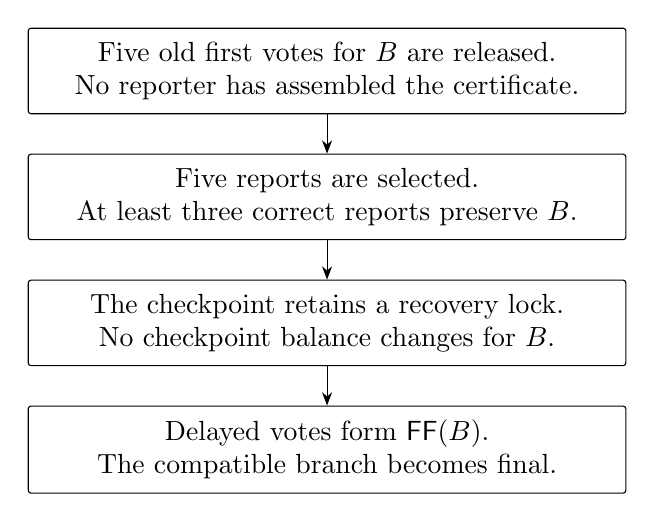
\begin{tikzpicture}[node distance=5mm,box/.style={draw,rounded corners=1pt,align=center,text width=2.85in,inner sep=5pt,font=\normalsize},>=Stealth]
\node[box] (a) {Five old first votes for $B$ are released.\\No reporter has assembled the certificate.};
\node[box,below=of a] (b) {Five reports are selected.\\At least three correct reports preserve $B$.};
\node[box,below=of b] (c) {The checkpoint retains a recovery lock.\\No checkpoint balance changes for $B$.};
\node[box,below=of c] (d) {Delayed votes form $\FF(B)$.\\The compatible branch becomes final.};
\draw[->] (a)--(b);\draw[->] (b)--(c);\draw[->] (c)--(d);
\end{tikzpicture}
\caption{Latent finality is an obligation of released votes. Report freezes are local events, not an atomic global stop.}
\Description{A four-stage vertical sequence: old first votes are released, selected frozen reports expose sufficient support, a checkpoint carries a recovery lock without balance effects, and delayed votes later form a final certificate.}
\label{fig:latent}
\end{figure}

The example generalizes in two ways. Every selected report quorum intersects a normal final-vote quorum in at least $p+1$ correct signers, each of whom recorded notarization before final-voting. Every selected report quorum intersects a fast first-vote quorum in at least $f+p+1$ correct signers, whose obligations occur in either the ledger set or $G_i$. These are the two exposure cases used by the closure theorem.

\subsection{Three responsibilities at the boundary}
Account voting determines certificate-backed finality. Closure determines the state and locks that any successor must preserve and may mark a uniquely retained closing-epoch notarized prefix for checkpoint finality. Agreement decides which valid candidate is installed; only that decision gives the marked prefix final effect. Agreement on a digest cannot compensate for missing report data or a construction that drops latent obligations.

The old committee validates reconstructed reports and a fixed evidence manifest before authorizing a candidate. The successor repeats those checks before installation. Meanwhile, its known membership allows preparation and first voting. Settlement before closure is deliberately narrower: the selected unresolved prefix must carry the required old- and new-epoch notarizations. This permits useful overlap without treating speculative successor votes as a veto on the predecessor checkpoint.

\section{Model and Guarantees}
\label{sec:model}
\subsection{Participants, faults, and retained evidence}
Clients own accounts and sign blocks. An authenticated committee contains $N=3f+2p+1$ equal-weight validator identities, where $f,p\geq0$ are integers. At most $f$ members of each committee are Byzantine. Corruption is globally static: adversarial identities are fixed throughout the execution, and a correct departing identity is not later compromised. Membership admission, Sybil resistance, and preservation of the per-committee fault bound are deployment assumptions. Deterministic committee selection does not establish any of them.

Signatures are unforgeable and hashes collision resistant. Canonical encodings bind the network session and message domain. An account vote binds its epoch, committee, account, slot, vote type, block hash, and admission-witness digest. The witness identifies the anchor and evidence under which the vote was admitted; it cannot be replaced after signing. Checkpoint votes bind the handoff context and deciding committee. Distinct signatures by one identity never contribute twice to a quorum for the same block.

Correct validators persist their first vote and terminal state before releasing signatures. They retain blocks, signed votes, and finite dependency evidence, and relay them after local voting ends. A certificate is a deterministic local view of sufficient individually verified votes, not a separately gossiped protocol object. A retained item held by a correct validator eventually reaches every correct validator that needs it. Departing validators continue service until correct successors hold durable copies. Epoch labels alone do not protect against stolen old keys; adaptive or mobile corruption is outside the model.

\begin{table}[t]
\caption{Account and closure thresholds. The example has $f=p=1$ and $N=6$.}
\label{tab:thresholds}
\centering
\begin{tabularx}{\columnwidth}{@{}Ylc@{}}
\toprule
Evidence & Threshold & Example\\
\midrule
Notarization $\NC$ & $q=N-f-p$ & 4\\
Normal finality $\FC$ & $q$ final votes & 4\\
Fast finality $\FF$ & $N-p$ first votes & 5\\
Recovery support & $r=f+p+1$ & 3\\
Selected reports & $N-f$ & 5\\
\bottomrule
\end{tabularx}
\end{table}

\subsection{Quorums and the role of \texorpdfstring{$p$}{p}}
The thresholds retained from the Kudzu-style voting construction are
\begin{align}
N&=3f+2p+1, &q&=2f+p+1, &r&=f+p+1.\label{eq:thresholds}
\end{align}
Table~\ref{tab:thresholds} distinguishes first, final, and report quorums. The parameter $p$ is the number of first-vote responses the fast path can omit, not an additional Byzantine-fault allowance. Increasing $p$ at fixed $f$ increases committee size. Normal progress needs $q$ responsive supporters; fast progress additionally needs $N-p$ timely first votes for the same block. We repeatedly use
\begin{align}
2q-N&=f+1,\label{eq:intersect}\\
q-2f&=p+1,\label{eq:normal-exposure}\\
(N-p)-2f&=f+p+1=r.\label{eq:fast-exposure}
\end{align}

\subsection{Accounts and canonical state}
Each account is a tree of owner-signed blocks rooted at genesis. A block's slot is one greater than its parent's slot. Slots are account positions, not times or retries. Blocks of one account conflict when neither is an ancestor of the other. An owner equivocates by signing conflicting blocks. Safety covers such owners; liveness does not promise a winner under persistent contention.

A closed checkpoint is $S_e=(L_e,\Sigma_e)$. The ledger $L_e$ identifies finalized prefixes, retained unresolved branches, and lock records. A lock record includes its block hash, strength (notarization or recovery), and the epoch whose potential finality it protects. Provenance matters: a certificate in an unrelated epoch cannot silently discharge an older lock. The application state $\Sigma_e$ contains balances, received-send identifiers, and applied-operation identifiers. A block is final either from an eligible account $\FC/\FF$ or because a decided checkpoint promoted it under Section~\ref{sec:build}; an undecided candidate has no finality effect.

Let $F_e$ be the finalized block set represented by $L_e$. A validator additionally maintains a certified live overlay $O_i$, containing locally finalized blocks not yet in $F_e$. Its effective final set is $F_e\cup O_i$, and its live application view is the deterministic replay of that set. The union is parent- and final-dependency-closed. Section~\ref{sec:install} defines installation without rolling back or reissuing its effects. A deterministic function derives $C_e$ from $\Sigma_e$, never from a private overlay. Later exposure of compatible finality cannot retroactively change $C_e$.

\subsection{Latent finality and progress assumptions}
\begin{definition}[Latent and late finality]
For a fixed epoch and admission context, a block is latent-final at a cut if released signatures and valid dependency evidence suffice to verify an eligible $\FC$ or $\FF$ for it or a descendant selecting it. Late finality is such a proof assembled or exposed after reports freeze or a checkpoint is decided. A closure obligation also covers a certificate completed by subsequent old-epoch signatures from identities that have not stopped.
\end{definition}
An outcome is eligible only under the attachment rules of Section~\ref{sec:account}; a large tally for provisional work is not account finality. Preservation requires retaining the selected branch or a compatible finalized extension. Checkpoint promotion is permitted only for a uniquely retained prefix already protected by closing-epoch notarization.

Safety has no message-delay bound. Progress requires finite relevant admitted work, fair processing and retry, retained-data availability, and recurring sufficiently long bounded-delay windows. In a prepared window, $\delta$ bounds message delivery and processing. Correct clock rates lie in $[1-\rho,1+\rho]$, where $0\leq\rho<1$. These assumptions are separated in Table~\ref{tab:assumptions}. An uncontested continuation has no conflicting owner-signed alternative at any new position, including signatures created earlier. Merely stopping new equivocation is insufficient.

\begin{table*}[t]
\caption{Assumption-to-guarantee map. None of the progress premises is a throughput or resource-isolation guarantee.}
\label{tab:assumptions}
\begin{tabularx}{\textwidth}{@{}p{1.10in}Yp{2.16in}@{}}
\toprule
Premise & Required condition & Guarantees using it\\
\midrule
Safety model & Static Byzantine identities; at most $f$ per committee; authentication; persistent voting; valid ancestry and prefix-wide eligibility. & Account exclusion and cross-epoch safety.\\
Data service & Correct holders retain and eventually serve blocks, votes, frozen reports, and committed candidate inputs. & Report usability and successor installation.\\
Finite preparation & The relevant admitted closing-epoch evidence is finite; reconstruction and semantic validation are fairly scheduled. & Eventual reconstruction and finite $\Build$.\\
Agreement progress & Recurring prepared windows with $N-f$ responsive correct old members, including catch-up and a correct-leader opportunity. & Handoff termination.\\
Account progress & Available dependencies; common-open ready intervals; persistent uncontested submission with retry or fresh-child continuation. & Account finality and eventual checkpoint inclusion.\\
\bottomrule
\end{tabularx}
\end{table*}

\section{Account-Local Processing}
\label{sec:account}
\subsection{Blocks, operations, and validation}
A block is $B=(a,h_p,x,\sigma_a)$: account, parent hash, ordered operation batch, and owner signature. Its identifier is
\[
h(B)=H(\mathsf{Block},a,h_p,x).
\]
The epoch is deliberately absent from this identifier, allowing a nonfinal omitted block to be retried with new-epoch votes. An empty batch is permitted for owner-authorized branch continuation. The two operations are $\Send(b,z)$, for destination $b$ and positive amount $z$, and $\Receive(s)$, where $s=(h(B),j)$ identifies a send at operation index $j$.

A send debits its owner. A receive credits only the named destination and requires an explicit proof that the send is already final. Transfer completion requires a final receive; the protocol does not create receives for passive recipients. These are separate owner-authorized operations, not an atomic update of two accounts.

Validation replays the entire unresolved selected path from its finalized anchor, then the proposed batch. It checks signatures, consecutive parent slots, destinations, positive amounts, balances, and duplicate receives using a temporary balance and received-send set. Checking each block only against the last finalized balance would miss a duplicate receive within an unresolved chain. Validation has no application effect. Every finalization repeats these checks and applies only previously unapplied operations.

A finality proof is either an account-certificate proof with the committee history, votes, attachment witnesses, and dependencies needed to verify eligibility, or a verified decided checkpoint that promoted the block. Proofs are finite, recursively verifiable evidence graphs; a circular reference is not a justification. A proof used for epoch-$e$ voting cannot depend on $S_e$ or a later checkpoint. A receive's send proof must be available before a correct validator supports the receiving path. These conditions make replay dependencies well founded (Lemma~\ref{lem:dag}).

\subsection{Single-support voting and durable state}
An account instance is $(\mathit{session},e,a,v)$. A correct validator first-votes at most once in that instance, for the first admissible available block it accepts. Its first vote is also its notarization support. There is no separate account notarization vote, no second-look support for a rival, and no account timeout vote.

A block is \emph{complete} in epoch $e$ when its data and required ancestry are available and the validator has assembled its epoch-$e$ $\NC$ from $q$ first votes. A complete block that is eligible is durably recorded as notarized before the validator final-votes, uses it as an eligible complete parent, or freezes its epoch report. The validator can final-vote only for its own first-voted block. It atomically records a terminal flag with that signature; it does not wait to observe an $\FC$ before remembering that voting ended.

An eligible block finalizes on $q$ final votes or $N-p$ first votes. Its selected unresolved ancestors finalize with it, and incompatible provisional branches are removed from the effective live view. An $\NC$ alone has no balance effect. Learning eligible finality closes the resolved voting instances, but relaying blocks and votes continues. A failed early attempt never resets an instance's first vote or terminal flag.

\para{Cross-epoch voting record.}
A correct identity stops epoch-$(e-1)$ signing before opening epoch $e$. While $S_{e-1}$ is unknown, it does not first-vote for a different block at a position where it first-voted in epoch $e-1$. Re-voting the same block is allowed. Once the predecessor is installed, its finalized history, frontier, and carried locks govern the position. This guard prevents a common identity from changing sides during overlap; the core protocol does not assume enough common identities to make that guard alone a quorum argument.

\subsection{Attachment and prefix-wide eligibility}
\label{sec:eligibility}
Let $d_a(S)$ be the maximum depth of any block for account $a$ retained in checkpoint $S$, including unresolved branches. With $S_{e-1}$ installed, a new epoch-$e$ root starts at depth $d_a(S_{e-1})+1$ and extends a maximum-depth retained tip. Subsequent children require complete epoch-$e$ parents. An extension must respect finalized history and every carried lock on its selected ancestry. A shorter retained branch cannot reopen a position below the frontier.

Before $S_{e-1}$ is known, first voting may prepare work from a maximum-depth tip of the latest closed ledger, from a closing-epoch finalized parent with its complete proof, or from a complete current-epoch parent. A closing-epoch notarized block may itself be re-voted when its parent is admissible. Such a block must also become complete in the current epoch before being used as a current-epoch complete parent. The signed admission-witness digest fixes the anchor and old evidence actually used; later rechecking cannot invent an earlier justification.

Ordinary early work is provisional. When the predecessor arrives, it is rechecked against the decided frontier, consecutive current-epoch parents, finalized history, and carried locks. A tally of fast-final size does not bypass this check. A notarization lock constrains settlement to its branch. A recovery lock can be discharged by a verified conflicting $\NC$ in the very epoch whose possible finality that lock protects: account exclusion then proves that its latent final certificate cannot exist. The discharge evidence is retained. A newer $\NC$ without this provenance is insufficient.

\para{The core overlap exception.}
A block may finalize before $S_{e-1}$ is known only if the verifier checks its entire selected prefix against the latest closed state and proves cross-boundary exclusion at \emph{every unresolved position being finalized}. Each such block, including the certificate target, must have a valid closing-epoch $\NC$ and a complete current-epoch $\NC$ for the same hash. A closing-epoch finalized prefix is already a safe anchor. Any inherited recovery lock bypassed by this path requires the matching-domain discharge proof above; inherited notarization locks cannot be bypassed.

Consequently, a descendant certificate can settle the selected prefix during overlap only when that descendant and all intervening unresolved blocks satisfy the same guard. A fresh descendant with no old-domain exclusion evidence remains provisional, even if its parent is notarized in both epochs. Otherwise disjoint committees could certify different children of that parent. This restriction sacrifices some overlap rather than deriving a cross-epoch exclusion result from a same-position parent certificate.

If the predecessor arrives first, nonfinal early work falls back to ordinary rechecking. Already finalized overlap work remains in the certified live overlay; installation cannot invalidate it. A decided checkpoint may promote only a uniquely retained closing-epoch notarized prefix; recovery-only uniqueness remains a lock. Supplement~B describes a possible alternative exclusion witness for fresh work, separately from this core rule.

\subsection{Fresh-child recovery}
If a checkpoint retains unresolved maximum-depth tips after the promotion rule, the owner can extend a permissible tip with a fresh child. Finalizing that child selects its unresolved ancestors rather than reopening their slots. A notarization or recovery lock still constrains the branch choice; the owner cannot use a child to evade an undischarged obligation.

This continuation policy is also needed for liveness. A block retained at the new frontier may no longer be a legal new root at its old position. Persistent submission therefore means retrying an omitted block, or supplying a fresh, possibly empty, uncontested child of a retained admissible tip. Repeatedly resubmitting the same locked block is not by itself a progress guarantee. Existing owner-signed conflicting children can still prevent the continuation from being uncontested.

\section{Safe Epoch Closure}
\label{sec:closure}
\subsection{Lagged committees and lifecycle}
The account committee for epoch $e$ is $K_e=C_{e-2}$. That old committee decides $S_e$; the already known successor $C_{e-1}=K_{e+1}$ verifies and installs it. The state $S_e$ derives $C_e$, whose account service starts in epoch $e+2$. Figure~\ref{fig:committees} separates selection, installation, and account voting. Genesis supplies $S_{-1}=S_G$ and $C_{-2}=C_{-1}=C_G$.

After local duration $D$, a validator may end epoch $e$ only when no older epoch remains closing. It stops old account signing, records all complete eligible old blocks as notarized, freezes its report against closed $S_{e-1}$, and opens $e+1$. Learning a decided checkpoint also stops any remaining signing for its closed epoch. Catch-up verifies predecessors in order and never reopens old vote records.

There is at most one closing epoch per validator. If closure outlasts $D$, the next local boundary is deferred. Successor voting can continue, subject to eligibility, but this is not a promise of uninterrupted settlement. The two-epoch lag gives future members an opportunity to synchronize, not a fixed upper bound on state transfer.

\begin{figure}[t]
\centering
\begin{tabularx}{\columnwidth}{@{}lYYY@{}}
\toprule
Account epoch & $e$ & $e+1$ & $e+2$\\
\midrule
Voters & $C_{e-2}$ & $C_{e-1}$ & $C_e$\\
Role for $S_e$ & Decide & Verify and install & Selected by $S_e$\\
\bottomrule
\end{tabularx}
\caption{Committee roles are logically staggered. Closure of $e$ can overlap account epoch $e+1$; the table does not impose synchronized wall-clock boundaries.}
\Description{A three-epoch table maps account voters to the committee that decides the checkpoint, the successor that verifies and installs it, and the future committee selected from its state.}
\label{fig:committees}
\end{figure}

\subsection{Immutable signed reports}
Every correct outgoing validator $i$ signs one header
\[
R_i=\Sign_i\bigl(\ctx_e,\Root(T_i),\Root(G_i)\bigr).
\]
The context binds the session, closing epoch, predecessor checkpoint, outgoing committee, and reporter identity. A Byzantine identity may equivocate, but a candidate selects at most one of its report headers.

Let $L_i$ be the reporter's ledger at freeze time. Its canonical tagged set is
\[
T_i=\{(h(B),s_i(B)):B\in L_i\},\qquad s_i(B)\in\{\tagR,\tagN,\tagF\}.
\]
An $\tagR$ entry is inherited recovery-protected state. An $\tagN$ entry has represented notarization but no locally observed finality. An $\tagF$ entry is final either by inherited checkpoint state or by an explicit account certificate for the block or a descendant selecting it. If several statuses hold, the strongest wins: $\tagF>\tagN>\tagR$. Inherited lock provenance comes from the verified predecessor; a new notarization is checked in its specified voting domain.

Let $V_i^{(e)}$ contain the hashes of all blocks for which $i$ released an epoch-$e$ account vote before freezing. The second committed set is
\[
G_i=V_i^{(e)}\setminus\keys(T_i).
\]
Thus the roots commit to ledger status and to voted-but-not-ledger membership, not to blocks or certificate objects. Correct reporters retain the frozen sets, vote records, and admission evidence. A later vote arrival, certificate assembly, or successor finalization can change their live view but cannot change the signed report.

\subsection{Reconstruction and report usability}
A root does not enumerate its members. Having all relevant block bodies is insufficient to know which tagged entries a reporter froze. Reconstruction is therefore a protocol precondition, not merely a bandwidth optimization.

For $T_i$, correct validators maintain a deterministic closing-epoch ledger projection, derived from the verified predecessor and retained relevant old-domain evidence. The projection excludes successor work and uses a canonical order and currently justified tags. Under finite relevant work and eventual gossip, correct validators converge to the same projection. Fair retry finds a root shared by requester and reporter. Because the reporter retained its frozen $T_i$, it can provide an authenticated difference from that common projection to its frozen set. The requester applies the difference and checks the signed target root.

The projection is an evidence-reconstruction view, not the validator's spendable live overlay. In particular, successor pruning cannot change the reference projection. The difference can insert and remove tagged entries and can approach the size of the whole committed set. There is no separate full-target fallback in this protocol.

After reconstructing $T_i$, the requester derives
\[
\widehat G_i=\{h(B):\text{$i$ signed an epoch-$e$ vote for $B$}\}\setminus\keys(T_i)
\]
from the reporter's retained signed votes. It accepts the set only when $\Root(\widehat G_i)=\Root(G_i)$. A missing outside-ledger vote prevents this check from succeeding. It then fetches blocks, ancestry, admission witnesses, and dependencies, and assembles the required $\NC$, $\FC$, or $\FF$ locally.

A report is usable only when both sets are reconstructed and its semantic claims are justified. An $\tagR$ entry must match predecessor recovery state; an $\tagN$ entry needs the relevant valid $\NC$ or inherited notarization record; an $\tagF$ entry needs valid inherited checkpoint finality or explicit account finality. A $G_i$ membership contributes reporter support only with $i$'s own first vote. Relaying another validator's vote never counts as reporter support. Provisional first-voted blocks remain distinguishable from eligible candidates. A Byzantine report with unavailable or malformed required material is unusable. Closure needs only $N-f$ usable reports, and at least that many reporters are correct.

\subsection{Immutable candidate inputs}
\label{sec:manifest}
The leader selects exactly $N-f$ usable report headers, in canonical identity order, forming $Q$. A candidate also commits to an evidence manifest $\mathcal M$, which lists content-addressed blocks, report reconstructions, exact supporting vote records, and finite admission and dependency witnesses. The corresponding bytes are retained protocol data; the manifest introduces no trusted certificate object.

The manifest removes an ambiguity between a committed report \emph{claim} and the evidence later chosen to validate that claim. Witness bytes are fixed before voting. The candidate value is
\[
v_e=(Q,\mu_e,d_e),\quad \mu_e=H(\mathcal M),\quad d_e=H(S_e),
\]
where $S_e=\Build(S_{e-1},Q,\mathcal M)$. A verifier must possess and validate the material addressed by $\mathcal M$. An extra private certificate can extend its live overlay, but cannot silently alter the candidate's construction input. A later proposal extending a certified candidate inherits both digests and $Q$.

The manifest is not a permission to omit required report material. Every selected membership, reporter vote, and needed ancestry witness must be covered. Nor may it promote an $\tagN$ or $G_i$ entry to final merely because an incidental final certificate is present. Final-output seeds are defined separately below. This separation makes the state digest a function of fixed semantic inputs rather than of certificate arrival order.

\subsection{Deterministic evidence summaries and locks}
\label{sec:build}
Let $\Anc(X)$ include $X$ and all its account ancestors. A candidate is an inherited block, a selected tagged block, or a block named by a selected $G_i$, together with the ancestors and fixed dependencies needed to validate it. Eligibility is checked against the closed predecessor or the explicit overlap evidence retained with its admission; an unexplained speculative path is excluded from new recovery counts. Recovery admissibility checks the required anchor, ancestry, dependencies, and cross-boundary witnesses, but does not require the candidate's own $\NC$ or final certificate; otherwise Rule~2 would be circular.

For a block $B$, let $\mathsf{f}_Q(B)$ mean that a selected $\tagF$ entry explicitly names $B$ and its finality witness verifies. Let $\mathsf{n}_Q(B)$ mean that selected $\tagN$ evidence represents an eligible notarization. Define the fresh reporter support set
\[
U_Q(B)=\{i:h(B)\in G_i\text{ and $\mathcal M$ verifies $i$'s first vote for $B$}\}.
\]
Inherited $\tagR$ entries add no fresh first-vote support. Finality witnesses can be for descendants, but only the named block and its selected ancestors are final-output seeds. An incidental witness-only descendant is not included just because its certificate proves an ancestor final.

\para{Final closure.}
Start with inherited finality and all blocks satisfying $\mathsf{f}_Q$. Take account-ancestor closure and recursively include the explicit finalized-send dependencies required by those final blocks. Every added send has a verified finality proof; the dependency is determined by the signed receive, not by a free choice of witness. Call the resulting set $F^\star$. Proof material for an unresolved receive does not by itself apply that receive or promote unrelated witness blocks. These rules make the application's finalized set independent of redundant proof encodings.

\para{Rule 1: represented notarization.}
At each new account position, after excluding conflicts with $F^\star$, retain the unique eligible represented $\NC$ target and its ancestry as a notarization lock. Same-domain account exclusion rules out two conflicting eligible $\NC$s. The lock constrains continuation, not balances.

\para{Rule 2: reporter first votes.}
If there is no represented eligible $\NC$ at that position and exactly one eligible block has $|U_Q(B)|\geq r$, retain that block and its ancestry as a recovery lock. Multiple threshold candidates do not cause an arbitrary winner or certificate-free finalization. The late-finality theorem shows that a genuinely formable fast-final block cannot coexist with such a threshold rival.

\para{Inherited state and discharge.}
Retain predecessor unresolved survivors unless explicit compatible finality excludes them or a matching-origin $\NC$ proves a recovery obligation impossible. Check lock discharge before permitting a conflicting new branch; do not infer it from a certificate's newer epoch number. If an inherited lock is already represented by a retained ancestor, preserve its provenance rather than counting it as fresh support. Newly named candidates below all thresholds need not be kept unless required by inherited state, an ancestor closure, or a validation dependency.

All evidence summaries are computed before any omission. Let $R_Q$ be the surviving inherited unresolved state, selected lock targets, and their required ancestor closure after finality and valid lock discharge. A block merely absent from competing selected evidence is not enough for finality.

\para{Rule 3: checkpoint promotion.}
For each account, starting at the tip of $F^\star$, repeatedly promote the next block only while (i) it is the unique child retained in $R_Q$ and (ii) the manifest verifies a closing-epoch $\NC$ for that block. Stop at the first fork or block without such an $\NC$. The resulting prefix $P_Q$ is only candidate-final until checkpoint agreement decides that candidate. Recovery-only blocks are never promoted by this rule. Let $F^+$ be the ancestor- and finalized-send-dependency closure of $F^\star\cup P_Q$; the output ledger marks $F^+$ final and retains $R_Q\setminus F^+$. Canonical sorting fixes serialization.

\begin{algorithm}[t]
\caption{\texorpdfstring{$\Build(S_{e-1},Q,\mathcal M)$}{BuildState}}
\label{alg:build}
\begin{algorithmic}[1]
\State Verify the predecessor, selected identities, report roots, and the committed manifest.
\State Reconstruct every selected $T_i,G_i$; verify the material for all required memberships and claims.
\State Form the parent-closed candidate set; classify admission and eligibility from fixed evidence.
\State Compute $F^\star$ by explicit-finality, ancestor, and finalized-send dependency closure.
\State Compute represented $\NC$ targets and reporter support sets for every position before pruning.
\State Check inherited locks and any matching-origin discharge witnesses; reject incompatible claims.
\State Apply Rules 1--2; retain inherited survivors and the ancestor closure of required lock targets, forming $R_Q$.
\State Apply Rule~3 to obtain candidate-final prefix $P_Q$; compute $F^+$ from $F^\star\cup P_Q$.
\State Retain $R_Q\setminus F^+$ and replay $F^+\setminus F_{e-1}$ once in canonical dependency order.
\State Return candidate $(L_e,\Sigma_e)$; Rule~3 has effect only if this candidate is decided.
\end{algorithmic}
\end{algorithm}

Replay orders parents before children and finalized sends before dependent receives. A promoted receive still uses the send-finality witness fixed when the receiving path was admitted; it cannot depend on the checkpoint being constructed. Among independent ready blocks, it chooses the lexicographically least $(a,v,h(B))$; within a block, it preserves the signed operation order. A cyclic or semantically invalid graph is rejected. Such rejection is not expected for an all-correct usable selection: the validity and acyclicity arguments establish a finite construction for that case. Algorithm~\ref{alg:build} specifies the order of validation, evidence summarization, lock selection, and replay.

\section{Checkpoint Agreement and Installation}
\label{sec:agreement}
\subsection{A contract over fixed candidates}
For handoff $e$, the closing committee invokes
\[
\Agree_{C_{e-2}}(\ctx_e,v_e).
\]
A decision returns a value and a publicly verifiable proof $\pi_e$. Candidate validity requires that $Q$ contain $N-f$ usable reports from distinct old members and that
\begin{align*}
H(\mathcal M)&=\mu,\\
\Build(S_{e-1},Q,\mathcal M)&=S\neq\bot,\\
H(S)&=d.
\end{align*}
All contexts, report identities, vote domains, and predecessor references must verify. Correct validators reconstruct and validate the full required input before authorizing a non-timeout proposal. Receiving a digest does not establish availability or validity.

The contract requires agreement and integrity: all valid decision proofs for one context identify the same value, and a proof cannot be replayed for another context. It requires external validity and retained availability of authorizing inputs. It requires conditional termination after enough valid immutable inputs become available during sufficiently long prepared progress windows. Rule~3 markings are hypothetical until this decision; $\pi_e$ makes them checkpoint-final. Finally, the successor installs only after independently verifying $\pi_e$ and recomputing the decided state.

A leader constructing a fresh candidate chooses $Q$ and $\mathcal M$. A proposal that extends a certified history inherits the entire payload; it cannot replace the report selection or evidence manifest. The specified instantiation uses one Kudzu-style vote instance over a checkpoint proposal history~\cite{kudzu}. Supplement~A records its election votes, timeout rules, and proof arguments. The main closure result depends on the contract rather than on those particular mechanics.

\subsection{Checkpoint base and certified live overlay}
\label{sec:install}
Let a validator's current closed base be $S_b$, with finalized set $F_b$, and let $O_i$ be its certified overlay. Its effective final set is $J_i=F_b\cup O_i$. Installing a verified successor checkpoint with final set $F_e$ computes
\[
J'_i=J_i\cup F_e,\qquad O'_i=J'_i\setminus F_e.
\]
The union is checked for account compatibility, final dependencies, and valid lock discharge. The validator adopts $S_e$ as its canonical base and materializes the live view as $\Replay(\Sigma_e,O'_i)$. This is a rebasing of a certified set of effects, not authorization to issue old sends again. Persistent operation identifiers suppress duplicate application and duplicate external notifications.

The installation invariant has three parts. The base's final set grows monotonically and may include checkpoint-promoted blocks. Every overlay block has an explicit account-finality proof for itself or a selecting descendant, and the union with the base is dependency-closed. Finally, that union extends each base-final account prefix and respects every undischarged notarization or recovery obligation. A recovery lock superseded by a matching-domain exclusion witness is removed from the effective view, not retroactively edited out of the signed checkpoint.

Committee $C_{e-1}$ does not hold a second election. It verifies the old committee's decision and reconstructs its state, derives $C_e$ from the canonical $\Sigma_e$, and rechecks nonfinal early work. Additional live finality never changes that committee selection. Invalidated provisional work is discarded without clearing its persisted first vote or terminal state. Already finalized overlap work remains certified and applied.

\section{Correctness}
\label{sec:correctness}
The arguments concern the core protocol, including the prefix-wide overlap guard and Rule~3 checkpoint promotion. They do not include the optional fresh-work extension of Supplement~B. Cryptographic guarantees hold except with negligible probability of forgery or collision. We first establish exclusion and report exposure, then deterministic closure and cross-epoch composition.

\subsection{Safety}
\begin{lemma}[Account exclusion]
\label{lem:exclusion}
In one account instance, at most one block has an $\NC$. An $\FC$ or $\FF$ excludes a conflicting $\NC$. If an $\FF$ is formable, every rival has at most $f+p<r$ first-vote supporters.
\end{lemma}
\begin{proof}
Two $q$-quorums intersect in at least $2q-N=f+1$ identities. At least one is correct and cannot first-vote for two blocks. An $\FC$ has a correct final voter who first obtained an $\NC$; an $\FF$ contains $N-p\geq q$ first votes. For the last claim, with actual Byzantine count $f'\leq f$, an $\FF$ has at least $N-p-f'$ correct first voters. At most $p$ correct identities remain for rivals; even adding all Byzantine identities gives at most $p+f'\leq p+f$ supporters for any rival.
\end{proof}

\begin{lemma}[Frozen-report exposure]
\label{lem:exposure}
A correct reporter's released final vote implies a frozen $\tagN$ or $\tagF$ entry for its selected block. Its first vote implies either a frozen ledger entry for that block or a membership in $G_i$. These statements persist after report creation.
\end{lemma}
\begin{proof}
Final voting follows durable eligible notarization. Account exclusion prevents incompatible same-domain finality from removing the selected path. The definition $G_i=V_i^{(e)}\setminus\keys(T_i)$ partitions the reporter's old-domain voted hashes. Stopping precedes freezing; roots and status tags then remain immutable. Authentication and retained admission witnesses preserve the corresponding semantic evidence.
\end{proof}

\begin{theorem}[Closure preserves latent and late finality]
\label{thm:closure}
Fix a valid closed predecessor. If an eligible old-epoch account final certificate can be formed, every valid checkpoint built from $N-f$ usable reports preserves its selected branch and ancestors, either as compatible finality or as the locks required by that certificate. The certificate may be assembled after report freeze or after checkpoint decision.
\end{theorem}
\begin{proof}
Let $R$ be the selected reporters. For a possible normal certificate with final-voter set $A$,
\[
|(R\cap A)\setminus\Byz|\ge q-2f=p+1.
\]
Each such correct reporter froze an $\tagN$ or $\tagF$ entry: $\tagF$ exposes finality and $\tagN$ triggers Rule~1. For a possible fast certificate,
\[
|(R\cap A)\setminus\Byz|\ge (N-p)-2f=r.
\]
Each of these reporters exposes the block through $T_i$ (as $\tagF$, $\tagN$, or inherited $\tagR$) or through $G_i$ with its verified first vote; in the latter case Rule~2 retains it. Lemma~\ref{lem:exclusion} prevents valid discharge or a threshold rival from eliminating genuine fast finality. Retained ancestry, admission evidence, and the committed manifest make these memberships usable. Later unselected or Byzantine signatures do not remove the required correct intersections.
\end{proof}

\begin{lemma}[Checkpoint-promotion safety]
\label{lem:promotion}
A Rule~3 promoted block cannot conflict with an eligible closing-epoch $\NC$, $\FC$, or $\FF$. Hence a decision that makes the promoted prefix final is compatible with old-domain finality and with core overlap finality.
\end{lemma}
\begin{proof}
Every promoted block has a verified closing-epoch $\NC$. Lemma~\ref{lem:exclusion} excludes a conflicting old $\NC$ and therefore conflicting old $\FC/\FF$. Core overlap finality for a conflicting successor block would itself require a conflicting closing-epoch $\NC$ at the first divergent position, also impossible. Promotion stops at retained forks and never promotes recovery-only evidence.
\end{proof}

\begin{lemma}[Acyclic final dependencies]
\label{lem:dag}
For any finite set of valid final blocks closed under account ancestors and required finalized sends, parent and send-to-receive edges form a directed acyclic graph.
\end{lemma}
\begin{proof}
Consider the earliest event at which valid final evidence can justify each block, including account certificates, checkpoint decisions, and justification by a descendant. Along a parent edge this event cannot become earlier at the child. Along a send-to-receive edge it is strictly later at the receive because admission already required the send's finality proof; Rule~3 cannot supply that proof for the checkpoint being constructed. A cycle cannot consist only of parent edges, because slots increase strictly. It must contain a send-to-receive edge, giving a strict increase around a cycle, a contradiction. Finite recursively verified evidence excludes circular certificates as an alternative justification.
\end{proof}

\begin{lemma}[Deterministic compatible construction]
\label{lem:construction}
Assume the predecessor satisfies the closure invariant. For fixed usable selected reports and a valid immutable manifest, $\Build$ returns one canonical candidate state. It preserves inherited finality, carries all mandatory surviving locks, and applies only explicit account finality plus Rule~3 checkpoint promotion. Correctly formed all-correct inputs yield a finite valid construction.
\end{lemma}
\begin{proof}
Fixed reports, witnesses, and proof choices fix explicit finality and $R_Q$. Lemma~\ref{lem:exclusion}, predecessor validity, attachment, and Theorem~\ref{thm:closure} make the retained finality and locks compatible. Rule~3's unique-child and verified-$\NC$ tests then fix $P_Q$, whose safety follows from Lemma~\ref{lem:promotion}. Lemma~\ref{lem:dag} and the canonical tie-break fix replay. Malformed Byzantine inputs may be rejected; all-correct usable inputs yield a finite state.
\end{proof}

\begin{theorem}[Transfer safety across epochs]
\label{thm:safety}
Assuming the checkpoint-agreement contract, finalized histories at correct validators are compatible and irreversible across all core-protocol epochs. Finalized balances are nonnegative, and each send is received at most once.
\end{theorem}
\begin{proof}
Induct from genesis. Lemma~\ref{lem:exclusion} excludes incompatible account finality; Theorem~\ref{thm:closure} preserves every eligible old final branch; Lemma~\ref{lem:promotion} makes checkpoint promotion compatible; and agreement installs only one verified state.

For overlap, the first divergent unresolved position on an early successor-final prefix has a closing-epoch $\NC$ for that successor block by the prefix-wide guard. A conflicting closing-epoch certificate, or a conflicting Rule~3 promotion, would require a conflicting $\NC$, contradicting Lemma~\ref{lem:exclusion}. Matching-origin discharge and inherited locks remain enforced. After installation, frontier and lock checks preserve this compatibility; base/overlay union and applied-operation identifiers prevent rollback or duplicate application. Replay checks balances and finalized-send dependencies, so balances stay nonnegative and each receive identifier is applied at most once.
\end{proof}

\subsection{Conditional termination}
\begin{lemma}[Correct reports become usable]
\label{lem:reports-live}
Under retained-data availability, finite relevant admitted work, and fair processing, retry, and eventual gossip, every correct report eventually becomes usable.
\end{lemma}
\begin{proof}
A correct reporter stops old signing, so its old vote set and roots are finite. Eventual delivery makes correct closing-epoch projections converge; fair retry reconstructs $T_i$, and retained signed votes reconstruct $G_i$. Available blocks, ancestry, and witnesses then complete finite validation. A withholding Byzantine reporter can make only its own report unusable; $N-f$ correct reports remain.
\end{proof}

\begin{theorem}[Handoff termination]
\label{thm:handoff-live}
Assume retained correct report data, fair processing, and recurring prepared progress windows with $N-f$ responsive correct old members, long enough for catch-up, input preparation, and the agreement contract. Every enabled handoff is eventually decided and, with eventual retained-data delivery, installed by correct successors.
\end{theorem}
\begin{proof}
Lemma~\ref{lem:reports-live} supplies usable reports and Lemma~\ref{lem:construction} a finite immutable candidate. The agreement contract decides it in a sufficient prepared window; retained authorizing data then let successors verify and install it, enabling the next deferred boundary.
\end{proof}

For the specified agreement instantiation, a sufficient local timeout condition is
\begin{equation}
\frac{\Delta_E}{1+\rho}>\kappa_E+\tau_E+\delta,\label{eq:election-window}
\end{equation}
where $\kappa_E$ bounds slot-entry skew and $\tau_E$ bounds proposal preparation and validation. A window must also cover catch-up and a complete correct-leader opportunity. This is a resource-and-timing premise, not a claim that short unrelated synchronous intervals suffice~\cite{dls}.

\begin{theorem}[Uncontested account continuation]
\label{thm:account-live}
Assume handoff termination, available final-send dependencies, and recurring common-open ready intervals. An owner following the retry-or-fresh-child policy of Section~\ref{sec:account} eventually finalizes each target of a finite valid uncontested continuation, provided each required new position has such an interval. The finalized targets eventually enter a checkpoint.
\end{theorem}
\begin{proof}
In a ready interval, $N-f\ge q$ correct first votes create an $\NC$ and the same validators can final-vote. An interrupted attempt is preserved by Theorem~\ref{thm:closure}; an omitted block can be retried, a uniquely retained notarized target may finalize at handoff, and any remaining retained fork can be selected by a fresh uncontested child. Repeating this argument over the finite continuation and using eventual evidence delivery gives finalization and checkpoint inclusion.
\end{proof}

With ancestry prepared, normal finality takes three delivery stages after broadcast: block, first votes, final votes. An available $N-p$ first-vote fast quorum takes two. A sufficient account interval budget is
\begin{equation}
\frac{D}{1+\rho}>\kappa_A+R_A+3\delta,\label{eq:account-window}
\end{equation}
where $\kappa_A$ bounds opening skew and $R_A$ bounds readiness after the last opening, including predecessor closure. Deferred boundaries only lengthen an open interval. These are conditional communication bounds, not measured latency.

\section{Costs, Scope, and Limitations}
\label{sec:costs}
\para{Agreement is not total system work.}
The agreed value contains $N-f$ report headers and two digests. With fixed-size identities and hashes, its reference portion is $O(N)$, independent of the number of account blocks. The evidence manifest, reconstruction data, validation, and retained histories are not constant size. They can scale with old state, new votes, and unresolved branches. Several proposal rounds can be necessary. One checkpoint per epoch means neither one agreement round nor constant reconfiguration cost.

\para{Account locality is not resource isolation.}
A correct validator releases at most one first vote and one final vote per account instance. This does not bound an adversary's owner-signed alternatives, network traffic, retained evidence, or validation work. A straightforward all-to-all vote dissemination has quadratic recipient deliveries in committee size per vote stage. No claim is made that RAI inherits Kudzu's erasure-coded communication bound or isolates accounts sharing physical resources.

\para{Overlap has an explicit frontier.}
Lagged committees permit preparation before closure. The core early-settlement path requires old-domain exclusion throughout the newly finalized prefix. New work without that evidence waits for the predecessor checkpoint; a long handoff can therefore delay finalization. A current $\NC$ for a fresh child does not protect it against an old committee's conflicting child. The optional predecessor-backed route requires additional temporal evidence and common members and is not part of the main theorem.

\para{Checkpoint promotion is narrow.}
A boundary decision may finalize a uniquely retained closing-epoch notarized prefix without an account $\FC/\FF$. It never promotes recovery-only state and does not provide continuous consensus or a general fork-resolution service.

\para{Retention and progress are conditional.}
Reports and validation manifests are compact commitments to potentially large data. A frozen-set difference can be nearly a full ledger-hash set. Forks and retained dependencies can accumulate without bound; the model supplies no general admission-control or garbage-collection policy. The finite-preparation assumption must be realized by a deployment rather than inferred from local signing limits. Departing validators cannot erase handoff evidence until successors durably hold it.

\para{Membership and finality have different state scopes.}
Committee derivation uses the checkpoint base, while an account's live view can include additional certified finality. This prevents later evidence from changing an already selected committee, but it means checkpoint-based membership does not instantly reflect all locally known finalized balances. The protocol is for authenticated committees with an externally maintained fault bound, not a complete permissionless staking or admission system.

\para{Security and expressiveness boundaries.}
The static adversary excludes later compromise of departed correct validators. Long-range security, mobile corruption, and forward-secure key management require separate designs and proofs. Account operations do not include general shared objects, atomic multiwriter transactions, passive-recipient credit, or a guaranteed winner under arbitrary equivocation. The proofs are written arguments rather than machine-checked verification. No empirical throughput, latency-under-load, or long-run resilience conclusion follows from them.

\section{Related Work}
\label{sec:related}
\subsection{Payments without a global execution order}
Guerraoui et al. characterize asset transfer's consensus number, including the single-owner case~\cite{consensusnumber}. FastPay provides prefunded Byzantine settlement without a global transaction order~\cite{fastpay}. Astro builds asynchronous payments on broadcast~\cite{astro}; Zef adds private coin payments and storage-conscious lifecycle mechanisms~\cite{zef}. Nano provides account-local chains and distinct send and receive operations~\cite{nano}. These precedents establish the application-level opportunity, not RAI's closure invariant. RAI does not claim that single-writer consensus avoidance, separate sends and receives, or account-local ordering is new.

Astro's extended version already discusses asynchronous replica reconfiguration using view-tagged messages and account-log transfer~\cite{astro,dbrb}. RAI's distinction is the frozen-report evidence used to preserve first- and final-vote obligations at its checkpoint boundary.

\subsection{Hybrid execution and contention recovery}
Sui Lutris uses consensus for shared objects and checkpoint sequencing, including End-of-Epoch handling of processed certificates~\cite{lutris}. RAI instead reconstructs account obligations from reports and does not continuously sequence ordinary certificates; these are different closure mechanisms under different application models.

Cuttlefish broadens the fast path with collective objects and multi-owner transactions, and uses FastUnlock to address contention~\cite{cuttlefish}. RAI's boundary promotion is narrower: it can finalize only a uniquely retained notarized account prefix at reconfiguration and does not provide a general consensus-backed resolution service for contested objects. Reduced expressiveness is a design boundary, not evidence of dominance.

\subsection{Dynamic membership and certificate boundaries}
Pastro studies permissionless asynchronous asset transfer with weighted stake and a dynamic adversary~\cite{pastro}; RAI instead assumes equal-weight authenticated committees and static corruption. Dynamic Byzantine Reliable Broadcast and asynchronous Byzantine reconfiguration address broader changing-participation settings~\cite{dbrb,reconfiguration}. RAI focuses on the account evidence needed for one agreed epoch checkpoint.

PDCC combines certificate-based payments with membership change and periodic settlement; its installation rule accepts certificates for the installed configuration and states a correct-member overlap assumption~\cite{pdcc}. RAI instead preserves eligible old-domain certificates that may be assembled later. The difference is boundary semantics, not a safety judgment about PDCC.

\begin{table*}[t]
\caption{Selected boundary mechanisms. This comparison concerns the cited designs, not measured performance or a completeness ranking.}
\label{tab:related}
\begin{tabularx}{\textwidth}{@{}p{0.84in}YY@{}}
\toprule
Design & Relevant mechanism & Distinction from the RAI core\\
\midrule
Astro~\cite{astro} & Asynchronous view changes and account-log transfer in the extended-version appendix. & Reconfiguration already exists; RAI studies its own frozen-report quorum obligations.\\
Sui Lutris~\cite{lutris} & Processed certificates enter consensus before End-of-Epoch handover. & RAI has no continuous account-certificate sequence to drain.\\
Pastro~\cite{pastro} & Permissionless asynchronous asset transfer with dynamic participation. & RAI's membership and corruption assumptions are narrower.\\
PDCC~\cite{pdcc} & Checkpoint-installed configurations and current-configuration certificate acceptance. & RAI's contract preserves eligible late old-domain finality.\\
RAI & Immutable reports, committed validation input, obligation locks, and narrow notarized-prefix promotion. & Account certificates finalize online; a decided checkpoint can also finalize a uniquely retained notarized prefix.\\
\bottomrule
\end{tabularx}
\end{table*}

\subsection{Agreement and authenticated reconstruction}
Simplex and Kudzu supply lightweight leader-based voting mechanisms~\cite{simplex,kudzu}. RAI reuses a Kudzu-style election only for checkpoint selection; its account path removes second looks and timeout support. The reconstruction layer uses authenticated commitments and differences as supporting mechanisms, not new cryptographic primitives. The protocol-specific requirement is that each frozen tagged ledger and voted-but-not-ledger set be reconstructible and semantically checkable. The preservation proof depends on those memberships and quorum intersections, not on an assumed compact difference or a particular authenticated-set implementation.

\section{Implementation and Evaluation}
\label{sec:eval}
\para{Prototype.}
We implemented RAI in RsNano~\cite{rsnano}, a Rust implementation of the Nano node~\cite{nano}. Account elections follow Section~\ref{sec:account} with the equal-weight thresholds of Table~\ref{tab:thresholds} ($f=p=1$, $N=6$). Epochs end at fixed times $T_0+kD$ on every validator. At a boundary each validator freezes a signed report; candidates are reconstructed from the selected reports, including a sketched authenticated difference when no root is shared, and the closing committee decides the checkpoint with a Kudzu-style election. Successors verify and install it off the vote-processing path. The prototype departs from the protocol of this paper in four ways. First, first votes, terminal states and retained evidence are held in memory; there is no durable signing record, so the runs below assume no crashes. Second, it implements the overlap exceptions of an earlier revision, which include the predecessor-backed route of Supplement~B, rather than the prefix-wide restriction of Section~\ref{sec:eligibility}. Third, the evaluated configuration disables checkpoint promotion: only certificate-backed finality is installed. Fourth, retained votes and blocks are kept for four epochs.

\para{Baseline.}
The baseline is unmodified RsNano (\texttt{develop}), which runs Nano's open representative voting: a block is confirmed once final votes reach 67\% of the online weight, after a first round of non-final votes. It has no epochs and no checkpoints. Final votes cannot be withdrawn, so a fork whose votes split can leave no side able to reach the quorum; the baseline gives no termination guarantee in that case, and its unresolved elections keep their slots in a bounded election container.

\para{Setup.}
All validators run as separate processes on one MacBook Air (Apple M1, eight cores, 16\,GiB, macOS~14.6) and communicate over loopback; LMDB runs without synchronous writes. Six equal-weight representatives hold the voting weight. A load generator funds 45{,}000 accounts and publishes 45{,}000 blocks at an offered 2{,}000 blocks/s, one block per account. With forks enabled, it publishes a conflicting sibling for 5\% or 10\% of the blocks, each sibling to half of the validators. An \emph{offline} validator runs no node and never votes but keeps its weight. A \emph{Byzantine} validator also runs no node; the generator votes with its key at random, choosing any vote type for recently published blocks and contradicting itself. Both arms use the same load-generator source; the binaries differ only in the vote encoding, since RAI votes carry their epoch. RAI uses 8\,s epochs, so a run spans three checkpoints. A run settles when every running validator holds the same cemented state and, for RAI, has decided the same checkpoints. We report non-fork blocks only: goodput is the number of non-fork blocks confirmed divided by the time from the start of publishing to the last such confirmation, and latency runs from a block's publication to its confirmation at one validator. The baseline's publishing phase may last 1.5 times RAI's longest publishing phase for the same variant; setup time is not counted. Each variant ran once per system on an otherwise idle machine. The baseline runs were taken in one pass; the RAI runs of Table~\ref{tab:eval} were taken in a second pass with the build that includes the two fixes described below, after an earlier pass with the build before them had exposed the defects.

\begin{table*}[t]
\caption{Non-fork goodput (blocks/s) and non-fork confirmation latency (ms) at an offered 2{,}000 blocks/s, one run per variant. With forks the non-fork share of the offered load is 95\% or 90\%. CP is the number of checkpoints every running validator decided identically. A baseline run that did not finish is given by the share of the 45{,}000 blocks confirmed when its publishing deadline expired.}
\label{tab:eval}
\centering
\begin{tabular}{@{}lrrrrrrrrc@{}}
\toprule
& \multicolumn{4}{c}{RsNano \texttt{develop} (no checkpoints)} & \multicolumn{5}{c}{RAI prototype (8\,s epochs)}\\
\cmidrule(lr){2-5}\cmidrule(l){6-10}
Variant & Blocks/s & p50 & p95 & p99 & Blocks/s & p50 & p95 & p99 & CP\\
\midrule
No forks & 1901 & 189 & 410 & 622 & 1934 & 101 & 205 & 309 & 3\\
No forks, 1 offline & 1907 & 207 & 238 & 285 & 1966 & 108 & 145 & 225 & 3\\
No forks, 1 Byzantine & 1921 & 205 & 234 & 289 & 1961 & 109 & 148 & 205 & 3\\
\midrule
5\% forks & \multicolumn{4}{c}{did not finish: 95.4\% confirmed} & 1799 & 124 & 591 & 805 & 3\\
5\% forks, 1 offline & \multicolumn{4}{c}{did not finish: 90.4\% confirmed} & 1828 & 116 & 254 & 468 & 3\\
5\% forks, 1 Byzantine & \multicolumn{4}{c}{did not finish: 93.0\% confirmed} & 1504 & 118 & 343 & 521 & 3\\
\midrule
10\% forks & \multicolumn{4}{c}{did not finish: 87.3\% confirmed} & 1332 & 267 & 1067 & 1384 & 3\\
10\% forks, 1 offline & \multicolumn{4}{c}{did not finish: 69.2\% confirmed} & 1357 & 139 & 1075 & 5280 & 3\\
10\% forks, 1 Byzantine & \multicolumn{4}{c}{did not finish: 86.4\% confirmed} & 1300 & 145 & 903 & 2678 & 3\\
\bottomrule
\end{tabular}
\end{table*}

\para{Without forks.}
Table~\ref{tab:eval} shows both systems keeping up with the offered load. RAI's goodput is 1.7--3.1\% higher and its median latency is about half the baseline's (101--109\,ms against 189--207\,ms), with lower p95 and p99. A likely cause is that an uncontested RAI block finalizes on one round of $N-p$ first votes, where the baseline needs a round of final votes after a quorum of non-final ones. One offline or Byzantine validator does not slow either system. With five running nodes instead of six, both use less of the shared CPU. Three checkpoints were decided on every running validator in all three variants, so closing epochs did not cost non-fork latency at this load.

\para{With forks.}
The baseline finished none of the six fork variants. In four of them the confirmation rate fell below 200 blocks/s 28--50\,s after publishing began and never recovered; in the other two it was still falling at the deadline. The confirmed share at the deadline ranged from 69\% to 95\%. Forks whose votes split stay unresolved and occupy election slots, which delays the non-fork blocks queued behind them. RAI finished and settled in all six fork variants, with three checkpoints decided identically on every running validator. With 5\% forks its median stayed at 116--124\,ms and its p95 at 254--591\,ms. With 10\% forks the median is 139--267\,ms and the p95 0.9--1.1\,s; the p99 reaches 5.3\,s with one offline validator, a handful of late confirmations. Between 0 and 718 forks were still undecided when publishing ended; they did not prevent settlement. Goodput falls with the fork rate, to 1{,}300--1{,}360 blocks/s at 10\%, since it is measured to the last non-fork confirmation and a few late blocks stretch that interval: in the 5\%-fork Byzantine run the last non-fork confirmation came 5\,s after the load generator finished, which lowers its goodput to 1{,}504 blocks/s while its latency percentiles are the lowest of the fork variants.

\para{Two defects found by the Byzantine fork workload.}
With 10\% forks and one Byzantine validator, a case within the fault model, the build before the fixes stalled: the epoch-2 checkpoint was never decided, confirmations nearly stopped 26\,s after publishing began with 43{,}575 of the 45{,}000 blocks confirmed, and the last non-fork block was confirmed 229\,s after publishing began. The cause was a mismatch between how an election forms a notarization certificate and how a validator checks one behind a report's $\tagN$ entry. An account election counts a final vote as notarization support as well, since a correct validator final-votes only what it notarized alone; the check against retained signed votes counted first and notarization votes only. A validator whose notarization leaned on a final vote, which the Byzantine validator casts at random, signed an $\tagN$ entry no other validator could verify, and with $N-f=5$ usable reports required of exactly five correct validators the checkpoint election could not start. Checking now counts the three vote kinds as the election does. The stall also exposed a cost: a solicitation named only the election's winner, so a validator holding the other candidate of a fork re-sent it every round to a requester that already held it, which dropped it on arrival after it had passed through the inbound queue. In the stalled run each validator sent 454{,}000 such candidates. Solicitations now name every candidate the requester holds, and a named candidate is not sent; the per-validator count fell to 2{,}750--7{,}200 across the fork variants, 3.5--13 times fewer than before the change. With both fixes the Byzantine 10\%-fork run decides all three checkpoints and settles in 86\,s, and at 10\% forks without faults the median fell from 502 to 267\,ms and the p95 from 4.2 to 1.1\,s. Neither defect is covered by the termination argument of Section~\ref{sec:correctness}: the first made a correct validator's report unusable, which the argument's assumption of retained correct report data rules out, and the second consumed the fair processing the argument takes for granted.

\para{Limitations.}
Each variant ran once, so the table gives no run-to-run variance. In earlier repeated runs of this prototype build, p95 varied by up to 40\% between identical runs, and the 5.3\,s p99 of the 10\%-fork offline variant is of that kind. All validators share one host, so CPU contention rather than network latency sets the delays, and the fixed offered load measures neither saturation capacity nor wide-area behavior. The baseline's deadline is relative to RAI's publishing time in the earlier pass; a longer deadline would raise its confirmed share but not end its stalled elections. The two arms were not interleaved in one pass, so slow host drift between the passes is not cancelled, though both passes ran on an idle machine and the goodput of the three no-fork RAI variants repeated within 0.5\% of the earlier pass. The prototype's in-memory signing records and its broader overlap rule mean these results do not validate the durability or the exact overlap restriction assumed by the proofs.

\section{Conclusion}
RAI separates online account finality, closure obligations, and checkpoint selection. Released votes can obligate a successor even when no correct process has assembled their final certificate. Immutable reports expose enough information to preserve those obligations; deterministic construction keeps recovery-only evidence nonfinal but lets a decided checkpoint promote a uniquely retained closing-epoch notarized prefix. Fixed validation inputs and a checkpoint-base/live-overlay invariant make reconstruction and installation explicit. Lagged committees allow preparation and carefully bounded dual-notarization overlap, while fresh work without old-domain exclusion waits for its predecessor checkpoint. A prototype in RsNano keeps non-fork latency near 100\,ms with three checkpoints per run and settles forked workloads, with one offline or one Byzantine validator, that the unmodified node does not finish; a Byzantine fork workload exposed a report-checking mismatch that the argument's assumptions do not tolerate, now repaired. The resulting core protocol supplies a precise safety boundary for reconfigurable single-writer payments under its stated fault, data, and progress assumptions.

\para{Use of AI tools.}
ChatGPT assisted with manuscript restructuring, source checking, protocol review, proposed specification changes, proof exposition, and LaTeX preparation. The changes include explicit validation-input commitments, a prefix-wide overlap restriction, narrow checkpoint promotion of uniquely retained notarized prefixes, and a separately scoped optional extension. Claude Code assisted with the prototype implementation, the benchmark harness, running the experiments, diagnosing the two defects, and drafting Section~\ref{sec:eval}. The proof arguments have not been machine checked and require author review.

\clearpage
\balance
\bibliographystyle{ACM-Reference-Format}
\bibliography{references}
\end{document}
